\section{Microservices}
In diesem Kapitel werden Mircoservices genauer betrachtet. Dazu wird zunächst der Zusammenhang zwischen DevOps und Mircoservices erläutert. Es wird gezeigt, dass Microservices optimal geeignet sind die Anforderungen von DevOps zu erfüllen. Daraufhin werden Architektur, Eigenschaften sowie Herausforderungen von Mircoservices vorgestellt. Dies wird immer unter dem Gesichtspunkt betrachtet, dass Microservices für DevOps eingesetzt wird. Dementsprechend werden stets die Punkte hervorgehoben, die für oder gegen den Einsatz in DevOps sprechen. Zum Schluss dieses Kapitels werden noch einige Gefahren und Antipattern vorgestellt.

\subsection{Motivation}

Entwicklerteams, die die DevOps Praktiken anwenden, sind üblicherweise sehr klein und haben geringe Koordination zu anderen Teams. Dadurch haben die Teams eine begrenzte Übersicht über die gesamte Anwendung. Sobald allerdings neu entwickelte Komponenten eingesetzt werden sollen, ist es zwingend notwendig Kompatibilität zu anderen Komponenten sicher zu stellen. Dies kann zum einen durch teamübergreifende Koordination oder durch den Einsatz einer bestimmten Architektur gelöst werden. \\
Des weiteren fordern die DevOps Praktiken das continuous Deployment. Dies sollte stets ohne große architektonische Anpassungen einsetzbar sein, um so die benötigte Zeit für die Einführung einer neuen Komponente möglichst gering zu halten. Weitere Anforderungen an die Architektur sind: Unterstützung unterschiedlicher Versionen einer Komponente, sodass Teammitglieder ohne größere Koordination eigene Neuentwicklungen einsetzen können. Ebenso sollen Rollbacks möglich sein, um zum einen live testing zu ermöglichen und im Fall von Fehlern die eingesetzte Komponente zurück zu setzten.\\

Diese Anforderungen werden allesamt von der Microservice Architektur erfühlt. Im folgenden Abschnitt wird diese Architektur genauer erläutert. 
 


\subsection{Architektur}

Bei der Mircroservice Architektur besteht die Softwareanwendungen beziehungsweise der Business Services aus mehreren kleinen Komponenten. Diese Komponenten werden Mircoservices genannt und beinhalten eine abgeschlossene kleine Funktion der Anwendung. Jede Komponente ist einzeln ausführbar, dies hat den Vorteil, dass für die Bereitstellung eines Mircoservices keine weiteren Komponenten benötigt werden und so keine beziehungsweise nur geringe Abhängigkeiten bestehen. Dementsprechend verfügen Microservices, sofern sie es benötigen, über ihre eigene Datenbank auf die nur sie zugreifen können. \\
Die Funktionen und Daten eines Mircoservices werden über das Interface des Mircoservices angeboten. Die Kommunikation zwischen den Microservices verläuft über das Netzwerk. Üblicherweise wird dafür ein simples Kommunikationsprotokoll wie HTTP verwendet. Der Aufruf eines oder mehrerer Microservices von einem Mircoservice bildet den gesamten Business Service. Abbildung \ref{aService} zeigt ein Beispiel. \\
Instanzen eines Services werden in einer Registry verwaltet und sobald ein Service eine Funktion eines anderen Services benötigt, fragt der Service bei der Registry nach diesem Service und erhält die benötigten Daten. Der genaue Ablauf der verschiedenen Akteure wird im folgenden Abschnitt genauer betrachtet.\\

\begin{figure}[htbp]
  \centering
  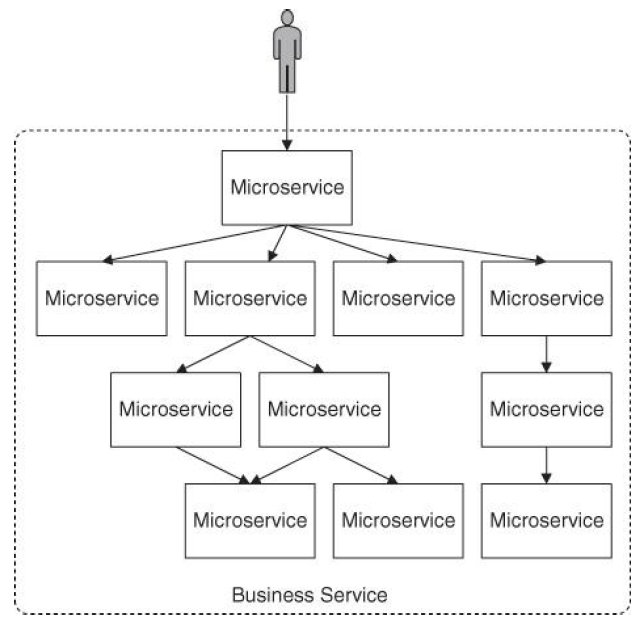
\includegraphics[width=0.5\textwidth]{pictures/businessService.png}
	\caption{Business service}
	\label{aService}
\end{figure}

\subsection{Design Entscheidung}
In diesem Abschnitt wird zunächst das Koordinationsmodell mit den drei Akteuren \textit{Client}, \textit{Service} und \textit{Registry/Load Balancer} vorgestellt. Daraufhin wird auf das Ressourcenmanagement von Instanzen eingegangen. Dazu werden Szenarien vorgestellt, die die Anzahl der Instanzen eines Microservices regulieren. Zum Schluss wird die Arbeitseinteilung und Zuweisung der architektonischen Elemente (Komponenten) erläutert. Dabei werden Möglichkeiten präsentiert, die die Microservice Architektur anbietet und daraufhin welche dieser Möglichkeiten für DevOps geeignet sind.

\subsubsection{Koordinationsmodell}

Beim Koordinationsmodell gibt es drei Akteure. Zum einen die \textit{Registry/Load Balancer}, wobei die Registry für die Verwaltung der Serviceinstanzen zuständig ist und der Load Balancer für die Verteilung der Last auf die verschiedenen Instanzen eines Services. So kann beispielsweise der Load Balancer bei erhöhter Anzahl von Anfragen auf einen Service weitere Instanzen anfordern, sodass Instanzen nicht überlastet werden.\\
Der zweite Akteur ist die \textit{Instanz eines Services}, die Daten beziehungsweise Dienstleistungen anbietet. Die Instanz registriert sich bei der Registry und hinterlegt ihren Namen, Adresse und Interface. Daraufhin steht nun die Instanz für den dritten Akteur bereit: Der \textit{Client} kann dabei ein Benutzer oder ein Service sein, der für einige Aufgaben weitere Services benötigt. Dafür fragt dieser bei der Registry nach den gewünschten Service und erhält die hinterlegten Daten der Serviceinstanz. Mit diesen Daten kann der Client nun die Instanz über das Interface ansprechen und verwenden. Die folgende Abbildung \ref{bService} gibt eine Übersicht der Beziehungen der drei Akteure.

\begin{figure}[htbp]
  \centering
  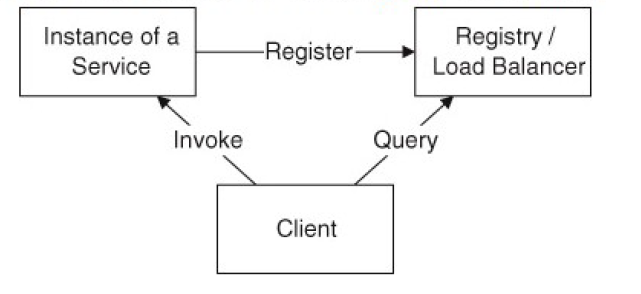
\includegraphics[width=0.5\textwidth]{pictures/3akteure.png}
	\caption{Die drei Akteure der Microservice Architektur}
	\label{bService}
\end{figure}

Da es jederzeit Möglich ist, dass Instanzen ausfallen können oder nicht mehr aktiv sind, ist es wichtig, dass die Registry über diese Instanzen informiert ist. Denn sonst vermittelt die Registry Instanzen an Clienten, die der Client nicht ansprechen kann. Für dieses Problem existiert der Healthcheck. Dabei werden Instanzen nur für eine bestimmte Zeit in der Registry verwaltet. Damit Instanzen nicht aus der Registry entfernt werden, müssen sich die Instanzen periodisch bei der Registry melden. Alternativ kann die Registry proaktive Anfragen an Instanzen stellen, die in der Registry registiert sind. Sollte die Instanz nach bestimmter Zeit keine Antwort liefern wird diese aus der Registry entfernt.

\subsubsection{Ressourcenmanagement}

Ein wichtiger Anforderungspunkt von DevOps ist die Skalierbarkeit. Weitere Serviceinstanzen lassen sich bei Ausfällen von Instanzen oder bei höhere Belastung initialisieren. Auch ist es möglich Instanzen bei geringerer Belastung zu entfernen um so Ressourcen zu sparen. Bei der Entscheidung, welcher Akteur über die Anzahl der Instanzen bestimmt, gibt es drei Szenarien:\\
Zum einen kann der Service selber entschieden ob er von sich weitere Instanzen bereitstellt, dies geschieht wenn der Service erkennt, dass Instanzen überbelastet sind. Zum Anderen kann der Client weitere Instanzen anfordern, sofern dieser bereits im Vorfeld weiss, dass er in naher Zukunft eine erhöhte Anzahl von Anfragen an einen Service hat. Im dritten Szenario kann eine externe Verwaltung durch Monitoring über die Anzahl der Instanzen entscheiden. So kann durch Monitoring erkannt werden, dass zu bestimmten Uhrzeiten ein Service vermehrt verwendet wird. Beispielsweise am Abend oder Wochenende, wo viele Benutzer zuhause sind und der Service von ihnen verwendet wird. 

\subsubsection{Abbildung von architektonischen Elementen}

Bei der Arbeitsaufteilung von Teams, können zum einen mehrere Teams einem Service arbeiten und ein Team an mehreren Services. Dies benötigt allerdings ein erhöhten Koordinationsaufwand. Idealerweise arbeiten an einem Service nur ein Team, wobei ein Team für mehreren Services zuständig sein kann. Dies entspricht auch den Anforderungen von DevOps, das geringe Koordination zwischen den Teams fordert.\\

Neben der Entwicklung einer Komponente von nur einem Team, sollen die Komponenten auch unabhängige Einheiten darstellen. So können diese unabhängig ausgeliefert werden und Änderungen haben keine Auswirkung auf andere Komponenten. Dies verringert ebenfalls die Koordination und beschleunigt die Auslieferung einzelner Komponenten. Die Anforderungen des continuous Deployment des DevOps werden damit ebenfalls erfüllt. 


\subsection{Herausforderungen}

Aufgrund der Eigenschaften, wie geringe Koordination zwischen Teams, hat die Architektur einige Herausforderungen. Dazu zählt zum einen die Systemstabilität und leichte Modifizierbarkeit der Module bei Erkennung von Problemen, wie beispielsweise neuen Versionen von benutzter Dritt-Software. Im folgenden werden die Herausforderungen der Microservicearchitektur genauer betrachtet.

\subsubsection{Systemstabilität}

Clienten sprechen Service über ein Interface an. Diese Interface können sich im Laufe der Entwicklung verändern. Aufgrund der geringen Koordination zwischen den Teams, können Missverständnisse bezüglich der Semantik vom Interface zwischen Client- und Service Team entstehen. So können Services mit neuen Interface einen unerwarteten Input erhalten, oder Clienten von einem Service mit neuen Interface ein unerwarteten Output. Um diesen Problemen entgegenzuwirken ist defensives Programmieren erforderlich, das heißt es benötigt eine große Anzahl unterschiedlicher Exceptions um die Fehler eingrenzen zu können. Zwar ist es möglich bei neuen Änderungen von Services Integrationstests durchzuführen, dies ist allerdings auf Grund der kurzen Releasephasen und der hohen Anzahl von Microservices sehr mühsam und Zeitaufwendig. Daher wird der \textit{Consumer driven contract} verwendet. Für jeden Microservices werden Testcases erstellt, die den Input und Output festlegen. Sobald die Interfacespezifikationen geändert werden, müssen die Testcases angepasst werden und von den Clienten, die den Service verwenden, akzeptiert werden. \\
Ein weitere Punkt für die Sicherstellung der Systemstabilität ist die Korrektheit der Umgebung. Systemumgebungen können fehlerhaft oder falsch konfiguriert sein. Damit der Service dennoch einwandfrei läuft muss bei der Initialisierung die Umgebung geprüft werden und gegebenenfalls muss sich der Service der Umgebung anpassen oder der Service passt die Umgebung an.\\
Ausfälle von Instanzen sind keine Seltenheit. Diese Ausfälle können mit Hilfe von Timeouts ermittelt werden und Clienten müssen alternative Mechanismen bei Timeout bereitstellen und ausführen. 

\subsubsection{Modifizierbarkeit}

Modifizierbarkeit bedeutet, dass Services leicht und schnell auf Änderungen angepasst werden können. Zwar ist es schwer ein Service so robust zu programmieren, dass auf jedes mögliche Problem schnell reagiert werden kann. Dennoch sollte der Service schnell die wahrscheinlichsten Änderungen identifizieren. Dazu gehört die Umgebung eines Services, das auf verschiedenen Rechnern unterschiedlich konfiguriert sein kann. Auch kann sich ein Zustand eines anderen verwendeten Services verändern. Das Interface sowie die angebotene Dienstleistung kann auf einer anderen Art bearbeitet werden, die möglicherweise mehr Zeit in Anspruch nimmt.\\
Neue Versionen von verwendete Bibliotheken und Dritt-Software können ebenfalls veränderte Funktionalität haben und so zu Problemen führen.\\
Da üblicherweise auf Identifizierte Veränderungen nicht direkt reagiert werden kann, wird versucht kaskadierende Effekte so gering wie möglich zu halten, sodass andere Bereiche nicht ebenfalls von den Problemen betroffen werden. Dazu werden mit Hilfe von Modulen die Änderungen gekapselt. Module sind in jeden Service enthalten und lokalisieren sowie isolieren Änderungen. Außerdem bieten die Module ein stabiles Interface zu den Änderungen an, sodass der Service möglichst normal weiterarbeiten kann. 

\subsection{Antipattern}

In diesem Abschnitt werden einige Antipattern vorgestellt und gezeigt wie die korrekte Vorgehensweise ist.

Funktionsumfang eines Services wächst mit der Zeit und den Anforderungen:\\
Services sollten möglichst klein gehalten werden und neu eingeführte Funktionen sollten jeweils ein neuen Service bilden.
Zu wenig Automatisierung der Test und des Deployments:\\
Um kurze Releasephasen einzuhalten ist es wichtig in allen möglichen Bereichen zu automatisieren, da sonst zu viel Zeit verloren geht.\\
Horizontale Schichten werden als Services abgebildet (z.B. Datenschicht und Geschäftslogik):\\
Microservices sollten möglichst unabhängig und einzeln ausführbar sein. Sobald Datenschicht und Geschäftslogik getrennt wird, benötigt mindestens ein Service für den Zugriff auf die Datenbank immer ein anderen Service. Dies entspricht nicht den gewünschten Eigenschaften von Microservices.\\
Jeder Service wird manuell konfiguriert:\\
Muss beispielsweise eine Internetadresse in den Servicen geändert werden, würde es sehr zeitaufwenig sein die Änderungen in jeden Service einzeln auszuführen. Daher sollten die Services mit einem Konfigurationsserver verbunden sein und Änderungen über diesen Server ausgeführt werden.\\
Zu jedem Service existiert nur eine Version:\\
Kurze Releasephasen bedeuten häufige Versionsänderungen. Existiert nur eine Version hat dies zur Folge, dass alle Instanzen der alten Version zerstört werden müssen. Dabei könnten diese Instanzen allerdings gerade von Clienten in Benutzung sein. Daher sollten nur Instanzen durch Serviceinstanzen der neuen Version ersetzt werden, wenn sie nicht verwendet werden.\\




\subsection{Gefahren}

Microservices beinhalten einige Gefahren. Die hohe Anzahl an Netzwerkverbindungen für die Kommunikation zwischen den Servicen, Clienten und der Registy kann zu mögliche Latenzen führen. Wodurch fälschlicherweise Timeouts ermittelt werden können. Auch verschlechtert sich die Effizienz des Business Services, da Clienten länger auf die Antwort eines Services warten muss.\\
Unerwartete Überlastungen von Serviceinstanzen verlangsamen die Performance. Ebenso führen Ausfälle von Instanzen zu geringerer Effizienz der gesamten Anwendung.\\
Bei einer hohen Anzahl von Serviceinstanzen kann es dazu kommen, dass die Registry nicht mit der Verwaltung der Instanzen hinter herkommt und es bei der Vermittlung der Instanzen an die Clienten zu Verzögerungen kommt oder sogar zur falschen Vermittlung einer Instanz.

\subsection{Beispiel}

Ein Beispiel für den Einsatz von Mircoservices ist Netflix. Ihr ganzes Streamingsystem ist auf der Microservicearchitektur aufgebaut. Durch die leichte Skalierbarkeit und Updaten von Microservices im laufenden Betrieb erreicht Netflix eine Verügbarkeitsquote von 99.7\%. Im Schnitt ist Netflix nur zwei Stunden im Monat nicht verfügbar.  
